\chapter{Elementos do texto}
\label{cap:texto}

Neste capítulo é dada uma visão geral sobre os elementos que podem ser utilizados no texto e código de inserção em \LaTeX.

% - - - - - - - - - - - - - - - - - - - - - - - - - - - - - - - - - - -
\section{Seccionamento de Documentos}
\label{sec:sec} 

O \LaTeX pode organizar, numerar e indexar capítulos e seções do documento. Existem até 7 níveis de profundidade para definir seções, dependendo da classe do documento:

\begin{quadro}[!ht]
\caption{Níveis de seccionamento de documentos em \LaTeX.}
\label{qua:niveis}
\begin{center}
\begin{tabular}{|c|c|}        
\hline
\textbf{Nível} & \textbf{Comando}\\ \hline\hline
-1 & \verb|\part| \\
\hline
0 & \verb|\chaper| \\
\hline
1 & \verb|\section| \\
\hline
2 & \verb|\subsection| \\
\hline
3 & \verb|\subsubsection| \\
\hline
4 & \verb|\paragraph| \\
\hline
5 & \verb|\subparagraph| \\
\hline
\end{tabular}
\end{center}
\fontequa{Elaborado pelo autor}
\end{quadro}

Para documentos com a \texttt{classe-ifg} utilize somente a partir do nível 0. Como exemplo, o código abaixo insere um capítulo que possui uma seção com uma subseção:

\begin{verbatim}
\chapter{Título do capítulo}
\label{cap:id}

Texto inicial do capítulo ...

\section{Título da seção}
\label{cap:sec}

Texto inicial da seção ...

\subsection{Título do subseção}
\label{cap:subsec}

Texto da subseção ...
\end{verbatim}

O comando \verb|\label| define um rótulo para fazer referência ao elemento rotulado. Como exemplo, este capítulo foi rotulado usando \verb|\label{cap:texto}|, de forma que o código \verb|Capítulo \ref{cap:texto}| produz Capítulo \ref{cap:texto}.

% - - - - - - - - - - - - - - - - - - - - - - - - - - - - - - - - - - -
\section{Listas}
\label{sec:listas} 

As listas são criadas definindo o tipo de lista e os itens que as formam, conforme descrito a seguir.

\subsection{Listas não ordenadas}

As listas não ordenadas (não numeradas) são produzidas pelo ambiente \verb|itemize|. Cada entrada deve ser precedida pelo comando \verb|\item|. A seguir está o código de uma lista não ordenada e o resultado produzido.

Código:

\begin{verbatim}
\begin{itemize}
    \item As entradas individuais são indicadas com um ponto preto, o 
denominado marcador.
    \item O texto nas entradas pode ter qualquer comprimento.
\end{itemize}
\end{verbatim}

Resultado:

\begin{itemize}
	\item As entradas individuais são indicadas com um ponto preto, o denominado marcador.
	\item O texto nas entradas pode ter qualquer comprimento.
\end{itemize}

\subsection{Listas ordenadas}

As listas ordenadas são geradas por um ambiente \verb|enumerate| e cada entrada deve ser precedida pelo comando \verb|\item|, que irá gerar automaticamente o número que rotula o item. Os rótulos enumerados consistem em números sequenciais; esses números começam em 1 com cada chamada para o ambiente enumerado.

Código:

\begin{verbatim}
\begin{enumerate}
    \item Os rótulos consistem em números sequenciais.
    \item Os números começam em 1 com cada chamada para o ambiente 
enumerado.
\end{enumerate}
\end{verbatim}

Resultado:

\begin{enumerate}
    \item Os rótulos consistem em números sequenciais.
    \item Os números começam em 1 com cada chamada para o ambiente enumerado.
\end{enumerate}

\subsection{Listas Aninhadas}

Em \LaTeX\ é possível inserir uma lista dentro de outra lista. As listas acima podem ser incluídas umas nas outras, misturadas ou de um tipo, em uma profundidade de quatro níveis.

Código:

\begin{verbatim}
\begin{enumerate}
    \item Os rótulos consistem em números sequenciais.
    \begin{itemize}
        \item As entradas individuais são indicadas com um ponto preto, 
o denominado marcador.
        \item O texto nas entradas pode ter qualquer comprimento.
    \end{itemize}
    \item Os números começam em 1 com cada chamada para o ambiente 
enumerado.
\end{enumerate}
\end{verbatim}

Resultado:

\begin{enumerate}
    \item Os rótulos consistem em números sequenciais.
    \begin{itemize}
      \item As entradas individuais são indicadas com um ponto preto, o denominado marcador.
      \item O texto nas entradas pode ter qualquer comprimento.
    \end{itemize}
    \item Os números começam em 1 com cada chamada para o ambiente enumerado.
\end{enumerate}

% - - - - - - - - - - - - - - - - - - - - - - - - - - - - - - - - - - -
\section{Figuras}
\label{sec:figs} 
Rótulos de figuras e tabelas devem ser centralizados se tiverem até uma linha (Figura~\ref{fig:exemploFig1}), caso contrário devem estar justificados e identados em ambas as margens, como mostrado na Figura ~\ref{fig:exemploFig2}. Essa formatação já é realizada automaticamente pela \textsf{classe-ifg}.

Os compiladores \LaTeX\ provêem um mecanismo bastante simples para inclusão de figuras, o que pode ser feito com o auxílio de várias classes auxiliares (as mais comuns são \verb|graphic| e \verb|graphicx|). A \textsf{classe-ifg} usa o comando \verb|\includegraphics|, da classe \verb|graphicx|, para a inclusão de figuras e não é necessário você colocar a extensão do arquivo neste comando. Por exemplo, para a figura \ref{fig:exemploFig1} os comandos usados foram:

\begin{verbatim}
\begin{figure}[ht!]
  \centering
  
\includegraphics[width=0.4\textwidth]{fig/logo-ifg-vertical-goiania}
  \caption{Logo IFG.}
  \label{fig:exemploFig1}
 \end{figure}
 \fontefig{\cite{ifg2020}}
\end{verbatim}

O código \verb|[ht!]| após \verb|\begin{figure}| define como a figura deve ser posicionada na página. O parâmetro especificador de posicionamento nos permite ter um maior controle sobre onde uma figura é colocada. Mas embora o \LaTeX\ faça o possível para seguir o posicionamento que especificamos, pode nem sempre ser possível aderir a ele. As opções possíveis são apresentadas na Tabela \ref{tab:pos}, sendo que pode ser especificado mais de um, o que indica que se um não for possível o próximo será tentado.

\begin{table}[ht!]
\caption{Especificadores de posicionamento no \LaTeX.}
\label{tab:pos}
\begin{center}
\begin{tabular}{c|p{11.5cm}}
\hline
\textbf{Especificador} & \textbf{Permissão} \\
\hline
\verb|h| & Coloque a figura aqui, ou seja, aproximadamente no mesmo ponto em que ocorre no texto de origem (no entanto, não exatamente no local) \\
\hline
\verb|t| & Posicione no topo da página. \\
\hline
\verb|b| & Posicione na parte inferior da página. \\
\hline
\verb|p| & Coloque em uma página especial somente com figuras.\\
\hline
\verb|!| & Substitua os parâmetros internos que o \LaTeX\ usa para determinar as posições adequadas.\\
\hline
\verb|H| &  Coloca a figura precisamente no local do código \LaTeX. Isso é um pouco equivalente a \verb|h!|, embora alguns erros possam surgir se você tiver muitos flutuadores consecutivos com \verb|[H]|.\\
\hline
\end{tabular}
\end{center}
\fontetab{Elaborada pelo autor}
\end{table}

O arquivo da figura deve ser inserido na pasta \verb|fig| e seu nome deve coincidir com o utilizado no comando \verb|\includegraphics|. O número inserido após \verb|width=| representa o tamanho da figura de maneira proporcional à largura do texto. Neste exemplo, \verb|0.4| significa 40\%. Dessa forma o valor máximo é \verb|1.0| (100\% da largura do texto).

O comando \verb|\fontefig| especifica a fonte de onde a figura foi retirada. Neste exemplo, foi utilizada uma figura de uma fonte externa, cuja descrição é descrita no documento \verb|bib/bibliografia.bib| usando o seguinte código:

\begin{verbatim}
@MISC{ifg2020,
  organization = {Instituto Federal de Educação, Ciência e Tecnologia 
de Goiás (IFG)}, 
  org-short = {IFG},
  year = {2020},
  title = {Apresentação}, 
  url = {http://ifg.edu.br/goiania/apresentacao},
  urlaccessdate = {07 nov 2020},
}
\end{verbatim}

Com isso, ao utilizar o comando \verb|\cite{ifg2020}| é criada uma citação a essa referência uma vez que \verb|ifg2020| foi usada como chave na descrição da fonte. Caso a figura tenha sido elaborada pelo próprio autor coloque \verb|\fontefig{Elaborada pelo autor}|. Note que nos dois casos não é necessário definir o ponto final pois ele é incluído automaticamente.


Ao se usar o compilador \LaTeX, as figuras podem estar nos formatos \textit{eps} e \textit{ps}. Ao se usar o PDF\LaTeX, as figuras podem estar nos formatos \textit{png}, \textit{jpg}, \textit{pdf} e \textit{mps}. A classe \verb|graphicx| também pode ser usada para a inclusão de figuras, nos formatos listados, ao se usar o PDF\LaTeX. Os comandos necessários são os mesmos ao se incluir figuras ao se usar o compilador \LaTeX. O uso do comando \verb|\includegraphics| faz com com que PDF\LaTeX\ procure primeiro por figuras com extensão \textit{pdf}, depois \textit{jpg}, depois \textit{mps} e por último \textit{png}. Aqui também não é necessário especificar a extensão do arquivo.

Para a inclusão das figuras \ref{fig:exemploFig1} à \ref{fig:exemploFig3} os comandos usados, tanto no \LaTeX\ quanto no PDF\LaTeX, seriam os mesmos. É claro que em cada caso devem estar disponíveis as figuras nos formatos suportados por cada compilador. Por exemplo, para a inclusão da figura \ref{fig:exemploFig3} foram usados:
\begin{verbatim}
 \begin{figure}[ht!]
  \centering
  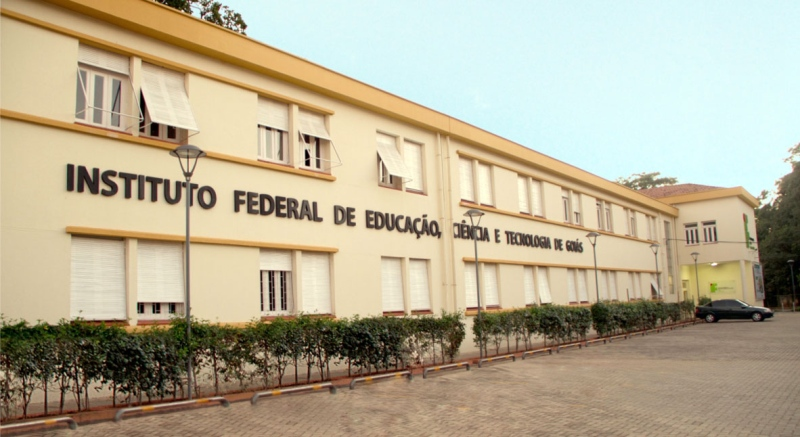
\includegraphics[width=0.40\textwidth]{./fig/foto-ifg}
  \caption{Câmpus Goiânia do IFG.}
  \label{fig:exemploFig3}
\end{figure}
\fontefig{\cite{ifg2020}}
\end{verbatim}

\begin{figure}[ht!]
 \centering
  
\includegraphics[width=0.30\textwidth]{./fig/logo-ifg-vertical-goiania}
 \caption{Logo IFG.}
 \label{fig:exemploFig1}
\fontefig{\cite{ifg2020}}
\end{figure}

\begin{figure}[ht!]
 \centering
 
\includegraphics[width=0.60\textwidth]{./fig/logo-ifg}
 \caption{Esta figura é um exemplo de um rótulo de figura que ocupa mais de uma linha, devendo ser identado e justificado.}
 \label{fig:exemploFig2}
\fontefig{\cite{ifg2020}}
\end{figure}

\begin{figure}[H]
 \centering
  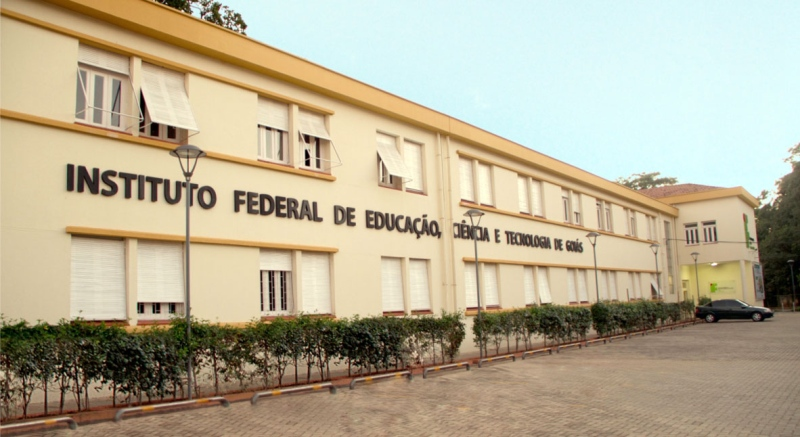
\includegraphics[width=0.70\textwidth]{./fig/foto-ifg}
  \caption{Câmpus Goiânia do IFG.}
 \label{fig:exemploFig3}
\fontefig{\cite{ifg2020}}
\end{figure}

\subsection{Subfiguras}
\label{subsec:subfigs} 

A classe \verb|subfigure| pode ser usada para a inclusão de figuras dentro de figuras (consulte a documentação da classe para maiores detalhes). Por exemplo, a Figura \ref{fig:subfiguras} contém duas subfiguras. Estas podem ser referencidas por rótulos independentes, ou seja, podem ser referenciadas como Figuras \ref{subfig:ex1} e \ref{subfig:ex2} ou Subfiguras \subref{subfig:ex1} e \subref{subfig:ex2}.
\begin{figure}[ht!]
 \centering
%   \subfigure[][Primeira subfigura.]
  \subfigure[][Primeira subfigura.]
   {
    
\includegraphics[width=0.35\textwidth]{./fig/triangulo}
    \label{subfig:ex1}
   } \qquad
  \subfigure[Segunda subfigura.]
   {
    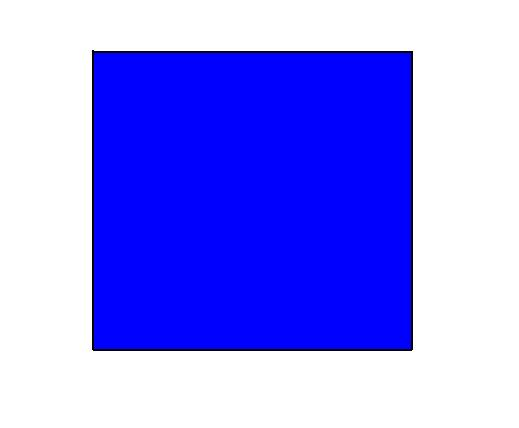
\includegraphics[width=0.30\textwidth]{./fig/quadrado}
    \label{subfig:ex2}
   }
   \caption{{\subref{subfig:ex1}} e {\subref{subfig:ex2}} representam dois exemplos do uso de subfiguras dentro de uma única figura.}
  \label{fig:subfiguras}
\fontefig{Elaborado pelo autor}
\end{figure}

A figura \ref{fig:subfiguras} foi incluída com os comandos listados a seguir. Observe que há rótulos independentes para cada uma das subfiguras e um rótulo geral para a figura, os quais podem ser todos referenciados. Dessa forma, os textos \aspas{Figuras \ref{subfig:ex1} e \ref{subfig:ex2}} ou \aspas{Subfiguras \subref{subfig:ex1} e \subref{subfig:ex2}} podem ser gerados utilizando os códigos \verb|Figuras \ref{subfig:ex1} e \ref{subfig:ex2}| ou \verb|Subfiguras \subref{subfig:ex1} e \subref{subfig:ex2}|.

\begin{verbatim}
\begin{figure}[ht!]
 \centering
  \subfigure[Primeira subfigura.]
   {
    \includegraphics[width=0.35\textwidth]{./fig/exemploFig1}
    \label{subfig:ex1}
   } \qquad
  \subfigure[Segunda subfigura.]
   {
    \includegraphics[width=0.30\textwidth]{./fig/exemploFig2}
    \label{subfig:ex2}
   }
   \caption{{\subref{subfig:ex1}} e {\subref{subfig:ex2}} representam
             dois exemplos do uso de subfiguras dentro de uma única
             figura.}
  \label{fig:subfiguras}
  \fontefig{Elaborado pelo autor}
\end{figure}
\end{verbatim}

\subsection{Figuras usando o pacote TikZ}

Figuras podem ser desenhadas diretamente em \LaTeX\ usando o pacote TikZ. Inicialmente é preciso definir o código da figura em um arquivo com a extensão \verb|tikz| que deve ser colocado na pasta \verb|fig|. Em seguida, a figura é inserida usando o comando \verb|inputTikZ| com o tamanho da figura.

Como exemplo, a Figura \ref{fig:tikz} foi inserida usando o código a seguir.

\begin{verbatim}
\begin{figure}[!ht]
 \centering
\inputTikZ{0.6}{./fig/exemplo.tikz}
\caption{Exemplo de figura usando o pacote TikZ.}
\label{fig:tikz}
\fontefig{Elaborada pelo autor}
\end{figure}
\end{verbatim}

\begin{figure}[!ht]
 \centering
\inputTikZ{0.6}{./fig/exemplo.tikz}
\caption{Exemplo de figura usando o pacote TikZ.}
\label{fig:tikz}
\fontefig{Elaborada pelo autor}
\end{figure}

O conteúdo do arquivo \verb|exemplo.tikz| é dado a seguir.

\begin{verbatim}
\begin{tikzpicture}[->,>=stealth',shorten >=1pt,auto,
node distance=3.8cm,thick,main node/.style={circle,draw,
font=\sffamily\bfseries,align=center,text width={1.5cm}}]

  \node[main node] (b) {$b$};
  \node[main node] (sales) [right of=b] {Depart. vendas};
  \node[main node] (ands1) [right of=sales,
  font=\sffamily\it] {\textit{AND$^s$}};
  \node[main node] (inventory) [above right of=ands1] 
  {Geren. invent{\'a}rio};
  \node[main node] (freight) [below right of=ands1] 
  {Escalon. de frete};
  \node[main node] (andj1) [below right of=inventory,
  font=\sffamily\it] {\textit{AND$^j$}};
  \node[main node] (crm) [below of=sales, 
  node distance=7.8cm] {CRM};
  \node[main node] (xors1) [right of=crm,
  font=\sffamily\it] {\textit{XOR$^s$}};
  \node[main node] (bank) [above right of=xors1] 
  {Sistema banc{\'a}rio};
  \node[main node] (payment) [below right of=xors1] 
  {Sistema pagamento};
  \node[main node] (xorj1) [below right of=bank,
  font=\sffamily\it] {\textit{XOR$^j$}};
  \node[main node, accepting, node distance=2.5cm] 
  (z) [right of=xorj1] {$z$};

  \path[every node/.style={font=\sffamily\small},
  align=center]
    (b) 			edge node {Submeter\\pedido} (sales)
    (sales) 		edge node {} (ands1)
    (sales) 		edge node [left] {Processar ordem\\ 
    de pagamento} (crm)
    (ands1) 		edge [bend left] node [above left]
    {Processar\\pedido} (inventory)
    (ands1) 		edge [bend right] node [below left] 
    {Escalonar\\frete} (freight)
    (inventory) 	edge [bend left] node {} (andj1)
    (freight) 		edge [bend right] node {} (andj1)
    (crm) 			edge node {} (xors1)
    (xors1) 		edge [bend left] node [above left] 
    {Enviar\\cobran\c{c}a\\: $p=0.3$} (bank)
    (xors1) 		edge [bend right] node [below left] 
    {Processar ordem\\ de pagamento\\: $p=0.7$} 
    (payment)
    (bank) 			edge [bend left] node {} (xorj1)
    (payment) 		edge [bend right] node {} (xorj1)
    (xorj1) 		edge node {} (z);
    
%\node[draw=none] at (0.0,-2.0) {$\lambda = 65$};
\end{tikzpicture}
\end{verbatim}
 
 %% - - - - - - - - - - - - - - - - - - - - - - - - - - - - - - - - -
\section{Tabelas}
\label{sec:tabs} 

Em tabelas, deve-se evitar usar cor de fundo diferente do branco e o uso de linhas grossas ou duplas. Ao relatar dados empíricos, não se deve usar mais dígitos decimais do aqueles que possam ser garantidos pela sua precisão e reprodutibilidade. Rótulos de tabelas devem ser colocados
antes das mesmas (veja a Tabela \ref{tab:MarcMNem}).

\begin{table}[ht!]
\caption{Conteúdo do diretório}
\label{tab:MarcMNem} 
\begin{center}
\begin{tabular}{c|c|c|c|c|c|c}
\hline Tag & Comprimento & Início &   & Tag & Comprimento & Início \\ 
\hline 001 & 0020 & 00000 && 100 & 0032 & 00235\\ 
\hline 003 & 0004 & 00020 && 245 & 0087 & 00267\\ 
\hline 005 & 0017 & 00024 && 246 & 0036 & 00354\\ 
\hline 008 & 0041 & 00041 && 250 & 0012 & 00390\\ 
\hline 010 & 0024 & 00082 && 260 & 0037 & 00402\\ 
\hline 020 & 0025 & 00106 && 300 & 0029 & 00439\\ 
\hline 020 & 0044 & 00131 && 500 & 0042 & 00468\\ 
\hline 040 & 0018 & 00175 && 520 & 0220 & 00510\\ 
\hline 050 & 0024 & 00193 && 650 & 0033 & 00730\\ 
\hline 082 & 0018 & 00217 && 650 & 0012 & 00763\\ 
\hline 
\end{tabular} 
\end{center}
\fontetab{\cite{Arm1979}}
\end{table}

A Tabela \ref{tab:MarcMNem} foi gerada usando o código a seguir.

\begin{verbatim}
\begin{table}[ht!]
\caption{Conteúdo do diretório}
\label{tab:MarcMNem} 
\begin{center}
\begin{tabular}{c|c|c|c|c|c|c}
\hline Tag & Comprimento & Início &   & Tag & Comprimento & Início \\ 
\hline 001 & 0020 & 00000 && 100 & 0032 & 00235\\ 
\hline 003 & 0004 & 00020 && 245 & 0087 & 00267\\ 
\hline 005 & 0017 & 00024 && 246 & 0036 & 00354\\ 
\hline 008 & 0041 & 00041 && 250 & 0012 & 00390\\ 
\hline 010 & 0024 & 00082 && 260 & 0037 & 00402\\ 
\hline 020 & 0025 & 00106 && 300 & 0029 & 00439\\ 
\hline 020 & 0044 & 00131 && 500 & 0042 & 00468\\ 
\hline 040 & 0018 & 00175 && 520 & 0220 & 00510\\ 
\hline 050 & 0024 & 00193 && 650 & 0033 & 00730\\ 
\hline 082 & 0018 & 00217 && 650 & 0012 & 00763\\ 
\hline 
\end{tabular} 
\end{center}
\fontetab{\cite{Arm1979}}
\end{table}
\end{verbatim}

O ambiente \verb|tabular| é usado para digitar tabelas. Para ficar mais claro sobre como funciona, a seguir está uma descrição de cada comando.

\begin{verbatim}
{c|c|c|c|c|c|c}
\end{verbatim}

Isso declara que sete colunas, separadas por uma linha vertical, serão usadas na tabela. Cada \verb|c| significa que o conteúdo da coluna será centralizado, você também pode usar \verb|r| para alinhar o texto à direita e \verb|l| para o alinhamento à esquerda.

\begin{verbatim}
\hline
\end{verbatim}

Isso irá inserir uma linha horizontal na tabela. Não há restrição quanto ao número de vezes que você pode usar \verb|\hline|.

\begin{verbatim}
cell1 & cell2 & cell3 & cell4 & cell5 & cell6 & cell7 \\
\end{verbatim}

Cada \& é um separador de células e a barra invertida dupla $\backslash\backslash$ define o final desta linha.

Outro exemplo é representado pela Tabela \ref{tab:outro}. O código para gerá-la é apresentado a seguir.

\begin{verbatim}
\begin{table}[h!]
\caption{Outro exemplo de tabela}
\label{tab:outro}
\renewcommand{\baselinestretch}{1.2}% for tabular environment
\small
\begin{center}
\begin{tabular}{cccccc}
\hline
   & \multirow{2}{22mm}{\renewcommand{\baselinestretch}{0.7}
   \small\centering Quantitative measures} & \multicolumn{4}{c}{Markers} 
   \\ \cline{3-6}
   & & \multicolumn{1}{c}{RO} & \multicolumn{1}{c}{ASF} & 
   \multicolumn{1}{c}{ISO} & \multicolumn{1}{c}{ADF} \\ \hline
   \multirow{3}{20mm}{\renewcommand{\baselinestretch}{0.7}
   \small\centering Test image scale 2}
& RMSE & 0.126 & 0.187 & 0.118 & 0.103 \\
& NMSE & 0.046 & 0.101 & 0.040 & 0.031 \\
& SSIM & 0.9981 & 0.9956 & 0.9984 & 0.9989 \\ \hline
   \multirow{3}{18mm}{\renewcommand{\baselinestretch}{0.7}\small
   \centering Cameraman scale 4}
& RMSE & 13.748 & 15.649 & 10.132 & 4.325 \\
& NMSE & 0.011 & 0.014 & 0.006 & 0.001 \\
& SSIM & 0.923 & 0.847 & 0.904 & 0.933 \\ \hline
\end{tabular}
\end{center}
\fontetab{Referência à fonte da tabela.}
\end{table}
\end{verbatim}

\begin{table}[h!]
\caption{Outro exemplo de tabela}
\label{tab:outro}
\renewcommand{\baselinestretch}{1.2}% for tabular environment
\small
\begin{center}
\begin{tabular}{cccccc}
\hline
   & \multirow{2}{22mm}{\renewcommand{\baselinestretch}{0.7}\small\centering Quantitative measures} & \multicolumn{4}{c}{Markers} \\ \cline{3-6}
   & & \multicolumn{1}{c}{RO} & \multicolumn{1}{c}{ASF} & \multicolumn{1}{c}{ISO} & \multicolumn{1}{c}{ADF} \\ \hline
   \multirow{3}{20mm}{\renewcommand{\baselinestretch}{0.7}\small\centering Test image scale 2}
& RMSE & 0.126 & 0.187 & 0.118 & 0.103 \\
& NMSE & 0.046 & 0.101 & 0.040 & 0.031 \\
& SSIM & 0.9981 & 0.9956 & 0.9984 & 0.9989 \\ \hline
   \multirow{3}{18mm}{\renewcommand{\baselinestretch}{0.7}\small\centering Cameraman scale 4}
& RMSE & 13.748 & 15.649 & 10.132 & 4.325 \\
& NMSE & 0.011 & 0.014 & 0.006 & 0.001 \\
& SSIM & 0.923 & 0.847 & 0.904 & 0.933 \\ \hline
\end{tabular}
\end{center}
\fontetab{Referência à fonte da tabela.}
\end{table}

Mais um exemplo de tabela é dado pela Tabela \ref{tab:maisum}, cujo código é apresentado a seguir.

\begin{verbatim}
\begin{table}[!ht]
\caption{Mais um exemplo de tabela}
\label{tab:maisum}
\renewcommand{\baselinestretch}{1.2}% for tabular environment
\small
\begin{center}
\begin{tabular}{ccccc}
\hline
\multirow{4}{16mm}{\renewcommand{\baselinestretch}{0.7}
\small\centering Leveling's Scale} & \multicolumn{4}{c}
{Values for the scale relation of the four different type of markers} 
\\ \cline{2-5}
& \multirow{3}{29mm}{\renewcommand{\baselinestretch}{1}\small
\centering Structure element's size $r$ for RO and ASF} & 
\multicolumn{2}{c}{Isotropic diffusion} & 
\multirow{3}{20mm}{\renewcommand{\baselinestretch}{1}\small
\centering Anisotropic diffusion iterations $t$} \\ \cline{3-4}
& & \multirow{2}{23mm}{\renewcommand{\baselinestretch}{0.7}
\small\centering Standard deviation $\sigma$} & \multirow{2}{12mm}
{\renewcommand{\baselinestretch}{0.7}\small\centering Kernel size} & \\
& & & & \\ \hline
1 & 1 & 0.5 & $5 \times 5$ & 100 \\
2 & 2 & 1.0 & $7 \times 7$ & 200 \\
3 & 3 & 1.5 & $11 \times 11$ & 300 \\
4 & 4 & 2.0 & $13 \times 13$ & 400 \\
5 & 5 & 2.5 & $17 \times 17$ & 500 \\
6 & 6 & 3.0 & $19 \times 19$ & 600 \\
7 & 7 & 3.5 & $23 \times 23$ & 700 \\ \hline
\end{tabular}
\end{center}
\fontetab{Referência à fonte da tabela.}
\end{table} 
\end{verbatim}

\begin{table}[!ht]
\caption{Mais um exemplo de tabela}
\label{tab:maisum}
\renewcommand{\baselinestretch}{1.2}% for tabular environment
\small
\begin{center}
\begin{tabular}{ccccc}
\hline
\multirow{4}{16mm}{\renewcommand{\baselinestretch}{0.7}\small\centering Leveling's Scale} & \multicolumn{4}{c}{Values for the scale relation of the four different type of markers} \\ \cline{2-5}
& \multirow{3}{29mm}{\renewcommand{\baselinestretch}{1}\small\centering Structure element's size $r$ for RO and ASF} & \multicolumn{2}{c}{Isotropic diffusion} & \multirow{3}{20mm}{\renewcommand{\baselinestretch}{1}\small\centering Anisotropic diffusion iterations $t$} \\ \cline{3-4}
& & \multirow{2}{23mm}{\renewcommand{\baselinestretch}{0.7}\small\centering Standard deviation $\sigma$} & \multirow{2}{12mm}{\renewcommand{\baselinestretch}{0.7}\small\centering Kernel size} & \\
& & & & \\ \hline
1 & 1 & 0.5 & $5 \times 5$ & 100 \\
2 & 2 & 1.0 & $7 \times 7$ & 200 \\
3 & 3 & 1.5 & $11 \times 11$ & 300 \\
4 & 4 & 2.0 & $13 \times 13$ & 400 \\
5 & 5 & 2.5 & $17 \times 17$ & 500 \\
6 & 6 & 3.0 & $19 \times 19$ & 600 \\
7 & 7 & 3.5 & $23 \times 23$ & 700 \\ \hline
\end{tabular}
\end{center}
\fontetab{Referência à fonte da tabela.}
\end{table} 

A Tabela \ref{tab:longas} é um exemplo de tabela longa que ocupa várias páginas. O código para incluí-la é apresentado a seguir, sendo omitido parte das linhas da tabela gerada.

\begin{verbatim}
\setlongtables
\begin{longtable}[c]{c|c|c|c|c|c}
\caption{Exemplo de tabela longa que atravessa várias páginas.}
\label{tab:longas}\\
\hline
\textbf{Campo1} & \textbf{Campo2} & \textbf{Campo3} & 
\textbf{Campo4} & \textbf{Campo5} & \textbf{Campo6} \\
\hline\hline
\endfirsthead
\caption[]{Continuação} \\
\hline
\textbf{Campo1} & \textbf{Campo2} & \textbf{Campo3} & 
\textbf{Campo4} & \textbf{Campo5} & \textbf{Campo6} \\
\hline\hline
\endhead
\hline\hline
\endlastfoot
\hline
\multicolumn{6}{r}{\captionlabelfont\captionsize(Continua)}\\
\endfoot
	campo1 & campo2 & campo3 & campo4 & campo5 & campo6 \\
	...
	campo1 & campo2 & campo3 & campo4 & campo5 & campo6 \\
\hline
\end{longtable}
% o comando \fontetab{} não pode ser usado neste caso
\vspace{-8mm}
\begin{center}
\footnotesize
Fonte: Referência a fonte da tabela.
\end{center}
\end{verbatim}

\setlongtables
\begin{longtable}[c]{c|c|c|c|c|c}
\caption{Exemplo de tabela longa que atravessa várias páginas.}
\label{tab:longas}\\
\hline
\textbf{Campo1} & \textbf{Campo2} & \textbf{Campo3} & \textbf{Campo4} & \textbf{Campo5} & \textbf{Campo6} \\
\hline\hline
\endfirsthead
\caption[]{Continuação} \\
\hline
\textbf{Campo1} & \textbf{Campo2} & \textbf{Campo3} & \textbf{Campo4} & \textbf{Campo5} & \textbf{Campo6} \\
\hline\hline
\endhead
\hline\hline
\endlastfoot
\hline
\multicolumn{6}{r}{\captionlabelfont\captionsize(Continua)}\\
\endfoot
	campo1 & campo2 & campo3 & campo4 & campo5 & campo6 \\
	campo1 & campo2 & campo3 & campo4 & campo5 & campo6 \\
	campo1 & campo2 & campo3 & campo4 & campo5 & campo6 \\
	campo1 & campo2 & campo3 & campo4 & campo5 & campo6 \\
	campo1 & campo2 & campo3 & campo4 & campo5 & campo6 \\
	campo1 & campo2 & campo3 & campo4 & campo5 & campo6 \\
	campo1 & campo2 & campo3 & campo4 & campo5 & campo6 \\
	campo1 & campo2 & campo3 & campo4 & campo5 & campo6 \\
	campo1 & campo2 & campo3 & campo4 & campo5 & campo6 \\
	campo1 & campo2 & campo3 & campo4 & campo5 & campo6 \\
	campo1 & campo2 & campo3 & campo4 & campo5 & campo6 \\
	campo1 & campo2 & campo3 & campo4 & campo5 & campo6 \\
	campo1 & campo2 & campo3 & campo4 & campo5 & campo6 \\
	campo1 & campo2 & campo3 & campo4 & campo5 & campo6 \\
	campo1 & campo2 & campo3 & campo4 & campo5 & campo6 \\
	campo1 & campo2 & campo3 & campo4 & campo5 & campo6 \\
	campo1 & campo2 & campo3 & campo4 & campo5 & campo6 \\
	campo1 & campo2 & campo3 & campo4 & campo5 & campo6 \\
	campo1 & campo2 & campo3 & campo4 & campo5 & campo6 \\
	campo1 & campo2 & campo3 & campo4 & campo5 & campo6 \\
	campo1 & campo2 & campo3 & campo4 & campo5 & campo6 \\
	campo1 & campo2 & campo3 & campo4 & campo5 & campo6 \\
	campo1 & campo2 & campo3 & campo4 & campo5 & campo6 \\
	campo1 & campo2 & campo3 & campo4 & campo5 & campo6 \\
	campo1 & campo2 & campo3 & campo4 & campo5 & campo6 \\
	campo1 & campo2 & campo3 & campo4 & campo5 & campo6 \\
	campo1 & campo2 & campo3 & campo4 & campo5 & campo6 \\
	campo1 & campo2 & campo3 & campo4 & campo5 & campo6 \\
	campo1 & campo2 & campo3 & campo4 & campo5 & campo6 \\
	campo1 & campo2 & campo3 & campo4 & campo5 & campo6 \\
	campo1 & campo2 & campo3 & campo4 & campo5 & campo6 \\
	campo1 & campo2 & campo3 & campo4 & campo5 & campo6 \\
	campo1 & campo2 & campo3 & campo4 & campo5 & campo6 \\
	campo1 & campo2 & campo3 & campo4 & campo5 & campo6 \\
	campo1 & campo2 & campo3 & campo4 & campo5 & campo6 \\
	campo1 & campo2 & campo3 & campo4 & campo5 & campo6 \\
	campo1 & campo2 & campo3 & campo4 & campo5 & campo6 \\
	campo1 & campo2 & campo3 & campo4 & campo5 & campo6 \\
	campo1 & campo2 & campo3 & campo4 & campo5 & campo6 \\
	campo1 & campo2 & campo3 & campo4 & campo5 & campo6 \\
	campo1 & campo2 & campo3 & campo4 & campo5 & campo6 \\
	campo1 & campo2 & campo3 & campo4 & campo5 & campo6 \\
	campo1 & campo2 & campo3 & campo4 & campo5 & campo6 \\
	campo1 & campo2 & campo3 & campo4 & campo5 & campo6 \\
	campo1 & campo2 & campo3 & campo4 & campo5 & campo6 \\
	campo1 & campo2 & campo3 & campo4 & campo5 & campo6 \\
	campo1 & campo2 & campo3 & campo4 & campo5 & campo6 \\
	campo1 & campo2 & campo3 & campo4 & campo5 & campo6 \\
	campo1 & campo2 & campo3 & campo4 & campo5 & campo6 \\
	campo1 & campo2 & campo3 & campo4 & campo5 & campo6 \\
	campo1 & campo2 & campo3 & campo4 & campo5 & campo6 \\
	campo1 & campo2 & campo3 & campo4 & campo5 & campo6 \\
	campo1 & campo2 & campo3 & campo4 & campo5 & campo6 \\
	campo1 & campo2 & campo3 & campo4 & campo5 & campo6 \\
	campo1 & campo2 & campo3 & campo4 & campo5 & campo6 \\
	campo1 & campo2 & campo3 & campo4 & campo5 & campo6 \\
	campo1 & campo2 & campo3 & campo4 & campo5 & campo6 \\
	campo1 & campo2 & campo3 & campo4 & campo5 & campo6 \\
	campo1 & campo2 & campo3 & campo4 & campo5 & campo6 \\
	campo1 & campo2 & campo3 & campo4 & campo5 & campo6 \\
	campo1 & campo2 & campo3 & campo4 & campo5 & campo6 \\
	campo1 & campo2 & campo3 & campo4 & campo5 & campo6 \\
	campo1 & campo2 & campo3 & campo4 & campo5 & campo6 \\
	campo1 & campo2 & campo3 & campo4 & campo5 & campo6 \\
	campo1 & campo2 & campo3 & campo4 & campo5 & campo6 \\
	campo1 & campo2 & campo3 & campo4 & campo5 & campo6 \\
	campo1 & campo2 & campo3 & campo4 & campo5 & campo6 \\
	campo1 & campo2 & campo3 & campo4 & campo5 & campo6 \\
	campo1 & campo2 & campo3 & campo4 & campo5 & campo6 \\
	campo1 & campo2 & campo3 & campo4 & campo5 & campo6 \\
	campo1 & campo2 & campo3 & campo4 & campo5 & campo6 \\
	campo1 & campo2 & campo3 & campo4 & campo5 & campo6 \\
	campo1 & campo2 & campo3 & campo4 & campo5 & campo6 \\
\hline
\end{longtable}
% o comando \fontetab{} não pode ser usado neste caso
\vspace{-8mm}
\begin{center}
\footnotesize
Fonte: Referência a fonte da tabela.
\end{center}

A \autoref{tab:longa} é um exemplo de tabela no modo paisagem e que ocupa também várias páginas. O código para incluí-la é apresentado a seguir, sendo omitido parte das linhas da tabela gerada.

\begin{verbatim}
\setlongtables
\begin{landscape}
\begin{longtable}[c]{c|c|c|c|c|c|c|c|c|c}
\caption{Exemplo de tabela longa, em paisagem, que atravessa 
várias páginas.}\label{tab:longa}\\
\hline
\textbf{BOX1} & \textbf{BOX2} & \textbf{BOX3} & \textbf{BOX4} & 
\textbf{BOX5} & \textbf{BOX6} & \textbf{BOX7} & \textbf{BOX8} & 
\textbf{BOX9} & \textbf{BOX10} \\
\hline\hline
\endfirsthead
\caption[]{Conclusão}\\
\hline
\textbf{BOX1} & \textbf{BOX2} & \textbf{BOX3} & \textbf{BOX4} & 
\textbf{BOX5} & \textbf{BOX6} & \textbf{BOX7} & \textbf{BOX8} & 
\textbf{BOX9} & \textbf{BOX10} \\
\hline\hline
\endhead
\endlastfoot
\hline
\multicolumn{10}{r}{\captionlabelfont\captionsize(Continua)}\\
\endfoot
	
	BOX1 & BOX2 & BOX3 & BOX4 & BOX5 & BOX6 & BOX7 & BOX8 
	& BOX9 & BOX10 \\
	...
	BOX1 & BOX2 & BOX3 & BOX4 & BOX5 & BOX6 &	BOX7 & BOX8 
	& BOX9 & BOX10 \\
\hline
\end{longtable}
\vspace{-8mm}
% o comando \fontetab{} não pode ser usado neste caso
\begin{center}
\footnotesize
Fonte: Referência a fonte da tabela.
\end{center}
\end{landscape}

\end{verbatim}

\setlongtables
\begin{landscape}
\begin{longtable}[c]{c|c|c|c|c|c|c|c|c|c}
\caption{Exemplo de tabela longa, em paisagem, que atravessa várias páginas.}\label{tab:longa}\\
\hline
\textbf{BOX1} & \textbf{BOX2} & \textbf{BOX3} & \textbf{BOX4} & \textbf{BOX5} & \textbf{BOX6} & \textbf{BOX7} & \textbf{BOX8} & \textbf{BOX9} & \textbf{BOX10} \\
\hline\hline
\endfirsthead
\caption[]{Conclusão}\\
\hline
\textbf{BOX1} & \textbf{BOX2} & \textbf{BOX3} & \textbf{BOX4} & \textbf{BOX5} & \textbf{BOX6} & \textbf{BOX7} & \textbf{BOX8} & \textbf{BOX9} & \textbf{BOX10} \\
\hline\hline
\endhead
\endlastfoot
\hline
\multicolumn{10}{r}{\captionlabelfont\captionsize(Continua)}\\
\endfoot
	
	BOX1 & BOX2 & BOX3 & BOX4 & BOX5 & BOX6 & BOX7 & BOX8 & BOX9 & BOX10 \\
	BOX1 & BOX2 & BOX3 & BOX4 & BOX5 & BOX6 & BOX7 & BOX8 & BOX9 & BOX10 \\
	BOX1 & BOX2 & BOX3 & BOX4 & BOX5 & BOX6 & BOX7 & BOX8 & BOX9 & BOX10 \\
	BOX1 & BOX2 & BOX3 & BOX4 & BOX5 & BOX6 &	BOX7 & BOX8 & BOX9 & BOX10 \\
	BOX1 & BOX2 & BOX3 & BOX4 & BOX5 & BOX6 &	BOX7 & BOX8 & BOX9 & BOX10 \\
	BOX1 & BOX2 & BOX3 & BOX4 & BOX5 & BOX6 &	BOX7 & BOX8 & BOX9 & BOX10 \\
	BOX1 & BOX2 & BOX3 & BOX4 & BOX5 & BOX6 &	BOX7 & BOX8 & BOX9 & BOX10 \\
	BOX1 & BOX2 & BOX3 & BOX4 & BOX5 & BOX6 &	BOX7 & BOX8 & BOX9 & BOX10 \\
	BOX1 & BOX2 & BOX3 & BOX4 & BOX5 & BOX6 &	BOX7 & BOX8 & BOX9 & BOX10 \\
	BOX1 & BOX2 & BOX3 & BOX4 & BOX5 & BOX6 &	BOX7 & BOX8 & BOX9 & BOX10 \\
	BOX1 & BOX2 & BOX3 & BOX4 & BOX5 & BOX6 & BOX7 & BOX8 & BOX9 & BOX10 \\
	BOX1 & BOX2 & BOX3 & BOX4 & BOX5 & BOX6 &	BOX7 & BOX8 & BOX9 & BOX10 \\
	BOX1 & BOX2 & BOX3 & BOX4 & BOX5 & BOX6 &	BOX7 & BOX8 & BOX9 & BOX10 \\
	BOX1 & BOX2 & BOX3 & BOX4 & BOX5 & BOX6 &	BOX7 & BOX8 & BOX9 & BOX10 \\
	BOX1 & BOX2 & BOX3 & BOX4 & BOX5 & BOX6 &	BOX7 & BOX8 & BOX9 & BOX10 \\
	BOX1 & BOX2 & BOX3 & BOX4 & BOX5 & BOX6 &	BOX7 & BOX8 & BOX9 & BOX10 \\
	BOX1 & BOX2 & BOX3 & BOX4 & BOX5 & BOX6 &	BOX7 & BOX8 & BOX9 & BOX10 \\
	BOX1 & BOX2 & BOX3 & BOX4 & BOX5 & BOX6 &	BOX7 & BOX8 & BOX9 & BOX10 \\
	BOX1 & BOX2 & BOX3 & BOX4 & BOX5 & BOX6 &	BOX7 & BOX8 & BOX9 & BOX10 \\                                 
	BOX1 & BOX2 & BOX3 & BOX4 & BOX5 & BOX6 &	BOX7 & BOX8 & BOX9 & BOX10 \\
	BOX1 & BOX2 & BOX3 & BOX4 & BOX5 & BOX6 &	BOX7 & BOX8 & BOX9 & BOX10 \\
	BOX1 & BOX2 & BOX3 & BOX4 & BOX5 & BOX6 &	BOX7 & BOX8 & BOX9 & BOX10 \\
	BOX1 & BOX2 & BOX3 & BOX4 & BOX5 & BOX6 &	BOX7 & BOX8 & BOX9 & BOX10 \\
	BOX1 & BOX2 & BOX3 & BOX4 & BOX5 & BOX6 &	BOX7 & BOX8 & BOX9 & BOX10 \\
	BOX1 & BOX2 & BOX3 & BOX4 & BOX5 & BOX6 &	BOX7 & BOX8 & BOX9 & BOX10 \\
	BOX1 & BOX2 & BOX3 & BOX4 & BOX5 & BOX6 &	BOX7 & BOX8 & BOX9 & BOX10 \\
	BOX1 & BOX2 & BOX3 & BOX4 & BOX5 & BOX6 &	BOX7 & BOX8 & BOX9 & BOX10 \\
	BOX1 & BOX2 & BOX3 & BOX4 & BOX5 & BOX6 &	BOX7 & BOX8 & BOX9 & BOX10 \\
\hline
\end{longtable}
\vspace{-8mm}
% o comando \fontetab{} não pode ser usado neste caso
\begin{center}
\footnotesize
Fonte: Referência a fonte da tabela.
\end{center}
\end{landscape}

%% - - - - - - - - - - - - - - - -- - - - - - - - - - - - - - - - - -
\section{Algoritmos}
\label{sec:algor} 
Algoritmos devem ser representados no formato do Algoritmo \ref{alg:poten}, que foi descrito com o uso da classe \textsf{algorithm2e}. A rigor não é obrigatório o uso dessa classe, contudo o uso da mesma permite que seja gerada automaticamente uma lista de algoritmos.

\medskip
\begin{center}
\begin{minipage}{0.92\textwidth}
\begin{algorithm2e}[H]
 \DontPrintSemicolon
 \LinesNumbered
 \SetAlgoLined
 \BlankLine
 \Entrada{vetor $A[i\,.\,.\,j]$, inteiros não negativos $i$ e $j$.}
 \Saida{vetor $A[i\,.\,.\,j]$ ordenado.}
 \BlankLine
 $n \leftarrow j - i$.\;
 \eSe{$(n<4)$}
   {Ordene com $\leq 3$ comparações.}
   {Divida $A$ em $\lceil\sqrt{n}\,\,\rceil$ subvetores de comprimento máximo $\lfloor\sqrt{n}\,\rfloor$.\;
    Aplique $MSR$ a cada um dos subvetores.\;
    Intercale os subvetores.\;}
\caption{$MSR(A,i,j)$ \label {alg:poten}}
\end{algorithm2e}
\end{minipage}
\end{center}

O código utilizado para gerar o algoritmo é apresentado a seguir. A lista completa de palavras-chave é apresentada no Apêndice \ref{apend:algorithm2e}.

\begin{verbatim}
\medskip
\begin{center}
\begin{minipage}{0.92\textwidth}
\begin{algorithm2e}[H]
 \DontPrintSemicolon
 \LinesNumbered
 \SetAlgoLined
 \BlankLine
 \Entrada{vetor $A[i\,.\,.\,j]$, inteiros não negativos $i$ e $j$.}
 \Saida{vetor $A[i\,.\,.\,j]$ ordenado.}
 \BlankLine
 $n \leftarrow j - i$.\;
 \eSe{$(n<4)$}
   {Ordene com $\leq 3$ comparações.}
   {Divida $A$ em $\lceil\sqrt{n}\,\,\rceil$ subvetores de 
   comprimento máximo $\lfloor\sqrt{n}\,\rfloor$.\;
    Aplique $MSR$ a cada um dos subvetores.\;
    Intercale os subvetores.\;}
\caption{$MSR(A,i,j)$ \label {alg:poten}}
\end{algorithm2e}
\end{minipage}
\end{center}
\end{verbatim}

%% - - - - - -  - - - - - - - - - - - - - - - - - - - - - - - - - - -
\section{Códigos de Programa}
\label{sec:progs} 

Códigos de programa podem ser importados, mantendo-se a formatação original, conforme se pode ver no exemplo do Código \ref{code:prog1}. Este exemplo usa o ambiente \textsf{codigo}, definido na \textsf{classe-ifg}, que permite que uma lista de programas seja gerada automaticamente.

\begin{center}
 \begin{codigo}[H]
   \small
   \lstinputlisting[language=Matlab]{prog/retangular.m}
   \caption{\texttt{funcao\_retangular()} }
   \label{code:prog1}
  \end{codigo}
\end{center}

Para inserir o código coloque na pasta \verb|prog| o arquivo com o conteúdo a ser inserido. Depois utilize o código a seguir. Atualmente a \textsf{classe-ifg} permite formatar códigos das linguagens XML, Java, Matlab e Python.

\begin{verbatim}
\begin{center}
 \begin{codigo}[H]
   \small
   \lstinputlisting[language=Matlab]{prog/retangular.m}
   \caption{\texttt{funcao\_retangular()} }
   \label{code:prog1}
  \end{codigo}
\end{center}
\end{verbatim}

%% - - - - - - - - - - - - - - - - - - - - - - - - - - - - - - - - - - -
\section{Teoremas, Corolários e Demonstrações}
\label{sec:teor}
 O uso do ambiente \textsf{theorem} permite a escrita de teoremas, como no exemplo a seguir:
\begin{verbatim}
\begin{theorem}[Pitágoras]
Em todo triângulo retângulo o quadrado do comprimento
da hipotenusa é igual a soma dos quadrados dos
comprimentos dos catetos.
\end{theorem}
\end{verbatim}

O resultado é o mostrado a seguir:

\begin{theorem}[Pitágoras]
Em todo triângulo retângulo o quadrado do comprimento da hipotenusa é igual a soma dos quadrados dos comprimentos dos catetos.
\end{theorem}

Da mesma forma pode-se usar o ambiente \textsf{proof} para demonstrações de teoremas:
\begin{verbatim}
\begin{proof}
Para demonstrar o Teorema de Pitágoras \dots
\end{proof}
\end{verbatim}

Neste caso, o resultado é:
\begin{proof}
Para demonstrar o Teorema de Pitágoras \dots
\end{proof}

Além desses dois ambientes, estão definidos os ambientes \textsf{definition} (Definição), \textsf{corollary} (Corolário), \textsf{lemma} (Lema)), \textsf{proposition} (Proposição), \textsf{comment} (Observação).

%% - - - - - - - - - - - - - - - - - - - - - - - - - - - - - - - - -
\section{Referências e citações}

Em documentos acadêmicos podem existir as citações podem ser: \textbf{implícitas} quando as referências não fazem parte do texto ou \textbf{explícitas} quando o autor referente a citação é mencionado explicitamente na sentença. Nesse sentido, deve-se utilizar os comandos específicos para cada tipo de citação, ou seja, em citações explicitas deve-se usar o comando \verb|citeonline{}| e nas demais situações é usado o comando\verb|cite{}|. Alguns exemplos são apresentados no \autoref{qua:exemplo-citacao}.

\begin{quadro}[!ht]
\centering
\caption{Exemplos de citações no documento}
\label{qua:exemplo-citacao}
\begin{tabular}{|c|c|}        
\hline
\textbf{Código em \LaTeX} & \textbf{Código Compilado}\\ \hline\hline
\begin{minipage}[t]{8cm}
\vspace{5pt}
\begin{verbatim}
A ironia será assim uma ... proposta
por \citeonline{10520:2000:4.1-1}.
\end{verbatim}
\vspace{5pt}
\end{minipage}
&
\begin{minipage}[t]{6cm}
\vspace{5pt}
A ironia será assim uma ... proposta 
por \citeonline{10520:2000:4.1-1}.
\vspace{5pt}
\end{minipage}\\\hline

\begin{minipage}[t]{8cm}
\vspace{5pt}
\begin{verbatim}
\citeonline[p.~146]{10520:2000:4.2-2}
dizem que ... 
\end{verbatim}
\vspace{5pt}
\end{minipage}
&
\begin{minipage}[t]{6cm}
\vspace{5pt}
\citeonline[p.~146]{10520:2000:4.2-2} dizem que {...}
\vspace{5pt}
\end{minipage}\\ \hline

\begin{minipage}[t]{8cm}
\vspace{5pt}
\begin{verbatim}
``Apesar das ... da filosofia''
\cite[p.~293]{10520:2000:4.1-2}.
\end{verbatim}
\vspace{5pt}
\end{minipage}
&
\begin{minipage}[t]{6cm}
\vspace{5pt}
``Apesar das {...} da filosofia'' \cite[p.~293]{10520:2000:4.1-2}.
\vspace{5pt}
\end{minipage} \\ \hline

\begin{minipage}[t]{8cm}
\vspace{5pt}
\begin{verbatim}
Depois, ...  que prefiro
\cite{10520:2000:4.1-3}.
\end{verbatim}
\vspace{5pt}
\end{minipage}
&
\begin{minipage}[t]{6cm}
\vspace{5pt}
Depois, {...} que prefiro \cite{10520:2000:4.1-3}.
\vspace{5pt}
\end{minipage}\\ \hline
\end{tabular}
\fontequa{\cite{icmc-usp}}
\end{quadro}

Para especificar a página, seção ou capítulo consultado na referência é preciso acrescentá-lo entre colchetes com os comandos \verb|\cite[página]{}| ou \verb|\citeonline[página]{}|. O texto colocado entre colchetes aparecerá logo após o ano. Maiores informações sobre os comandos utilizados para citação posem ser consultados no manual de referência da abnTeX2, incluindo o uso de \textbf{apud} \cite{abntex2cite-alf}.

\section{Citações Indiretas}

As citações indiretas são caracterizadas como uma espécie de paráfrase das ideias de um determinado autor, ou seja, o pesquisador, por meio de suas próprias palavras, interpreta o discurso de outrem, contudo, mantendo o mesmo sentido. Outro aspecto que deve ser considerado é a necessidade de o autor (ou os autores) e o ano em que a obra foi publicada serem mencionados. 

Nas citações indiretas há duas formatações possíveis dependendo de como ocorre a citação no texto. Quando o autor é mencionado explicitamente utiliza-se o comando \verb|\citeonline{}|, caso contrário, deve utilizar o comando \verb|cite{}|. 

\section{Citações diretas}
\label{sec-citacao}

As citações diretas ocorrem quando o texto de uma referência é transcrito literalmente. As citações diretas curtas (até três linhas) são inseridas no texto entre aspas duplas. As aspas simples são utilizadas para indicar citação no interior da citação: \aspas{Nas citações, as chamadas pelo sobrenome do autor [...] incluído na sentença devem ser em letras maiúsculas e minúsculas e, quando estiverem entre parênteses, devem ser em letras maiúsculas} \cite[sec.~5]{NBR10520:2002}.

\begin{verbatim}
``Nas citações, as chamadas pelo sobrenome do autor [...] incluído na 
sentença devem ser em letras maiúsculas e minúsculas e, quando 
estiverem entre parênteses, devem ser em letras maiúsculas''
\cite[5]{NBR10520:2002}.
\end{verbatim}

Cabe ressaltar que em \LaTeX as aspas iniciais são diferentes das finais. Para tanto, pode-se utilizar o comando \verb|\aspas{CONTEUDO}| para inserir um determinado conteúdo entre aspas.

As citações diretas longas (com mais de 3 linhas) podem ser inseridas por meio do ambiente \texttt{citacao}:

\begin{citacao}
As citações diretas, no texto, com mais de três linhas, devem ser
destacadas com recuo de 4 cm da margem esquerda, com letra menor que a do texto
utilizado e sem as aspas. No caso de documentos datilografados, deve-se
observar apenas o recuo \cite[5.3]{NBR10520:2002}.
\end{citacao}

Use o ambiente assim:

\begin{verbatim}
\begin{citacao}
As citações diretas, no texto, com mais de três linhas [...] deve-se 
observar apenas o recuo \cite[5.3]{NBR10520:2002}.
\end{citacao}
\end{verbatim}

\section{Referências Bibliográficas}

As referências bibliográficas utilizadas neste modelo estão de acordo com a Norma Brasileira ABNT 6023:2018 Informação e documentação - Referências - Elaboração \cite{abnt}. A seguir são apresentados exemplos em cada um das categorias, considerando somente os elementos essenciais. Adicionalmente, é apresentado o código \BibTeX~para geração da referência.

\subsection{Monografia no todo}\label{sec:monografia}

Inclui livro e/ou folheto (manual, guia, catálogo, enciclopédia, dicionário, entre outros) e trabalho acadêmico (tese, dissertação, trabalho de conclusão de curso, entre outros).

Os elementos essenciais para livro e/ou folheto são: autor, título, subtítulo (se houver), edição (se houver), local, editora e data de publicação. Quando necessário, acrescentam-se elementos complementares à referência para melhor identificar o documento.

EXEMPLO 1

LUCK, Heloisa. \textbf{Liderança em gestão escolar}. 4. ed. Petrópolis: Vozes, 2010.

\begin{verbatim}
@book{luck2014e,
 author = {Heloisa Luck},
 title = {Liderança em gestão escolar},
 edition = {2},
 address = {Petrópolis},
 publisher = {Vozes},
 year = {2010}
}
\end{verbatim}

EXEMPLO 2

BAUMAN, Zygmunt. \textbf{Globalização}: as consequências humanas. Rio de Janeiro: Jorge Zahar, 1999.

\begin{verbatim}
@book{bauman99,
 author = {Zygmunt Bauman},
 title = {Globalização},
 subtitle = {as consequências humanas},
 address = {Rio de Janeiro},
 publisher = {Jorge Zahar},
 year = {1999}
}
\end{verbatim}

Os elementos essenciais para trabalho acadêmico são: autor, título, subtítulo (se houver), ano de depósito, tipo do trabalho (tese, dissertação, trabalho de conclusão de curso e outros), grau (especialização, doutorado, entre outros) e curso entre parênteses, vinculação acadêmica, local e data de apresentação ou defesa. Quando necessário, acrescentam-se elementos complementares à referência para melhor identificar o documento.

EXEMPLO 1

AGUIAR, André Andrade de. \textbf{Avaliação da microbiota bucal em pacientes sob uso crônico de penicilina e benzatina}. Tese (Doutorado em Cardiologia) — Faculdade de Medicina, Universidade de São Paulo, São Paulo, 2009.

\begin{verbatim}
@phdthesis{aguiar09,
 author = {André Andrade de Aguiar},
 title = {Avaliação da microbiota bucal em pacientes sob uso crônico de penicilina e benzatina},
 year = {2009},
 type = {Doutorado em Cardiologia},
 school = {Faculdade de Medicina, Universidade de São Paulo},
 address = {São Paulo}
}
\end{verbatim}

EXEMPLO 2

ALVES, Daian Péricles. \textbf{Implementação de conceitos de manufatura colaborativa}: um projeto virtual. Trabalho de Conclusão de Curso (Bacharelado em Engenharia Industrial Mecânica) — Universidade Tecnológica Federal do Paraná, Curitiba, 2008.

\begin{verbatim}
@tcc{alves08,
 author = {Daian Péricles Alves},
 title = {Implementação de conceitos de manufatura colaborativa},
 subtitle = {um projeto virtual},
 year = {2008},
 type = {Bacharelado em Engenharia Industrial Mecânica},
 school = {Universidade Tecnológica Federal do Paraná},
 address = {Curitiba}
}
\end{verbatim}

EXEMPLO 3 

RODRIGUES, Ana Lúcia Aquilas. \textbf{Impacto de um programa de exercícios no local de trabalho sobre o nível de atividade física e o estágio de prontidão para a mudança de comportamento}. Dissertação (Mestrado em Fisiopatologia Experimental) — Faculdade de Medicina, Universidade de São Paulo, São Paulo, 2009.

\begin{verbatim}
@mastersthesis{rodrigues09,
 author = {Ana Lúcia Aquilas Rodrigues},
 title = {Impacto de um programa de exercícios no local de trabalho sobre o nível de atividade física e o estágio de prontidão para a mudança de comportamento},
 year = {2009},
 type = {Mestrado em Fisiopatologia Experimental},
 school = {Faculdade de Medicina, Universidade de São Paulo},
 address = {São Paulo}
}
\end{verbatim}

EXEMPLO 4 

PANIAGO, Cecília Yade Nogueira Alves. \textbf{A relação entre professor-aluno na educação de jovens e adultos (EJA)}. Monografia (Especialização em Docência na Educação Profissional, Técnica e Tecnológica) — Instituto Federal de Educação, Ciência e Tecnologia de Goiás, Senador Canedo, 2020.

\begin{verbatim}
@monography{paniago20,
 author = {Cecília Yade Nogueira Alves Paniago},
 title = {A relação entre professor - aluno na educação de jovens e adultos (EJA)},
 year = {2020},
 type = {Especialização em Docência na Educação Profissional, Técnica e Tecnológica},
 school = {Instituto Federal de Educação, Ciência e Tecnologia de Goiás},
 address = {Senador Canedo}
}
\end{verbatim}

\subsection{Monografia no todo em meio eletrônico}

Para documentos em meio eletrônico, as referências devem obedecer aos padrões indicados para os documentos monográficos no todo, de acordo com a Seção~\ref{sec:monografia}, acrescidas da descrição do endereço eletrônico.

EXEMPLO 1 

BAVARESCO, Agemir; BARBOSA, Evandro; ETCHEVERRY, Katia Martin. \textbf{Projetos de filosofia}. Porto Alegre: EDIPUCRS, 2011. Disponível em: http://ebooks.pucrs.br/edipucrs/projetosdefilosofia.pdf. Acesso em: 21 ago. 2011.

\begin{verbatim}
@book{bavaresco11,
 author = {Agemir Bavaresco and Evandro Barbosa and Katia Martin Etcheverry},
 title = {Projetos de filosofia},
 year = {2011},
 address = {Porto Alegre},
 publisher = {EDIPUCRS},
 url = {http ://ebooks.pucrs.br/edipucrs/projetosdefilosofia.pdf},
 urlaccessdate = {21 ago. 2011}
}
\end{verbatim}

EXEMPLO 2

COELHO, Ana Cláudia. \textbf{Fatores determinantes de qualidade de vida física e mental em pacientes com doença pulmonar intersticial}: uma análise multifatorial. Dissertação (Mestrado em Ciências Médicas) — Faculdade de Medicina, Universidade Federal do Rio Grande do Sul, Porto Alegre, 2009. Disponível em: http://www.lume. ufrgs.br/bitstream/handle/10183/16359/000695147.pdf?sequence=1. Acesso em: 4 set. 2009.

\begin{verbatim}
@mastersthesis{coelho09,
 author = {Ana Cláudia Coelho},
 title = {Fatores determinantes de qualidade de vida física e mental em pacientes com doença pulmonar intersticial},
 subtitle = {uma análise multifatorial},
 year = {2009},
 type = {Mestrado em Ciências Médicas},
 school = {Faculdade de Medicina, Universidade Federal do Rio Grande do Sul},
 address = {Porto Alegre},
 url = {http://www.lume.ufrgs.br/bitstream/handle/10183/16359/000695147.pdf?sequence=1},
 urlaccessdate = {4 set. 2009}
}
\end{verbatim}

\subsection{Parte de monografia}

Inclui secção, capítulo, volume, fragmento e outras partes de uma obra, com autor e/ou título próprios.

Os elementos essenciais são: autor e título da parte, seguidos da expressão \textit{In:}, e da referência completa da monografia no todo. No final da referência, deve-se informar a descrição física da parte. Quando necessário, acrescentam-se elementos complementares à referência para melhor identificar o documento.

EXEMPLO 1 

SANTOS, Fernando Rodrigues dos. A colonização da terra do tucujús. \textit{In}: \_\_\_\_. \textbf{História do Amapá, 1$^o$ grau}. 2. ed. Macapá: Valcan, 1994. cap. 3, p. 15–24.

\begin{verbatim}
@inbook{santos94,
 author = {Fernando Rodrigues dos Santos},
 booktitle = {História do Amapá, 1$^o$ grau},
 title = {A colonização da terra do Tucujús},
 chapter = {3},
 edition = {2},
 pages = {15-24},
 publisher = {Valcan},
 year = {1994},
 address = {Macapá}
}
\end{verbatim}

EXEMPLO 2 

ROMANO, G. Imagens da juventude na era moderna. \textit{In}: LEVI, G.; SCHMIDT, J. (Org.). \textbf{História dos jovens 2}: a época contemporânea. São Paulo: Companhia das Letras, 1996. p. 7–16.

\begin{verbatim}
@incollection{romano96,
 author = {G. Romano},
 booktitle = {História dos jovens 2},
 booksubtitle = {a época contemporânea},
 title = {Imagens da juventude na era moderna},
 editor = {G. Levi and J. Schmidt},
 editortype = {Org.},
 pages ={7-16},
 publisher = {Companhia das Letras},
 year = {1996},
 address = {São Paulo}
}
\end{verbatim}

\subsection{Publicação periódica}

Inclui o todo ou partes de: coleção, fascículo ou número de revista, jornal, entre outros.

\subsubsection{Coleção de publicação periódica}

A referência de toda a coleção de um título de periódico é utilizada em listas de referências e catálogos de obras preparados por livreiros, bibliotecas ou editoras.

Os elementos essenciais são: título, subtítulo (se houver), local de publicação, editora, datas de início e de encerramento da publicação (se houver), e ISSN (se houver). Quando necessário, acrescentam-se elementos complementares para melhor identificar o documento.

EXEMPLO 1 

REVISTA BRASILEIRA DE GEOGRAFIA. Rio de Janeiro: IBGE, 1939--. ISSN 0034-723X.

\begin{verbatim}
@book{geografia39,
 address = {Rio de Janeiro},
 issn = {0034-723X},
 organization = {Revista Brasileira de Geografia},
 publisher = {IBGE},
 year = {1939--}
}
\end{verbatim}

EXEMPLO 2 

ACTA CIRúRGICA BRASILEIRA. São Paulo: Sociedade Brasileira para o Desenvolvimento da Pesquisa em Cirurgia, 1997–. ISSN 1678-2674 versão \textit{online}. Disponível em: http://www.scielo.br/scielo.php?script=sci\_serial\&pid=0102-8650\&lng=pt\&nrm=iso. Acesso em: 22 ago. 2013.

\begin{verbatim}
@book{acta97,
 address = {São Paulo},
 issn = {1678-2674 versão \textit{online}},
 organization = {Acta Cirúrgica Brasileira},
 publisher = {Sociedade Brasileira para o Desenvolvimento da Pesquisa em Cirurgia},
 year = {1997--},
 url = {http://www.scielo.br/scielo.php?script=sci_ serial&pid=0102-8650&lng=pt&nrm=iso},
 urlaccessdate = {22 ago. 2013}
}
\end{verbatim}

\subsubsection{Artigo, seção e/ou matéria de publicação periódica}

Inclui partes de publicação periódica, artigo, comunicação, editorial, entrevista, recensão, reportagem, resenha e outros.

Os elementos essenciais são: autor, título do artigo ou da matéria, subtítulo (se houver), título do periódico, subtítulo (se houver), local de publicação, numeração do ano e/ou volume, número e/ou edição, tomo (se houver), páginas inicial e final, e data ou período de publicação.

EXEMPLO 1

COSTA, V. R. À margem da lei: o programa comunidade solidária. \textbf{Em Pauta} — Revista da Faculdade de Serviço Social da UERJ, Rio de Janeiro, n. 12, p. 131–148, 1998.

\begin{verbatim}
@article{costa98,
 address = {Rio de Janeiro},
 author = {V. R. Costa},
 journal = {Em Pauta},
 number = {12},
 pages = {131-148},
 section = {Revista da Faculdade de Serviço Social da UERJ},
 title = {À Margem da Lei: o Programa Comunidade Solidária},
 year = {1998}
}
\end{verbatim}

\subsubsection{Artigo e/ou matéria de jornal}

Inclui comunicação, editorial, entrevista, recensão, reportagem, resenha e outros.

Os elementos essenciais são: autor, título, subtítulo (se houver), título do jornal, subtítulo do jornal (se houver), local de publicação, numeração do ano e/ou volume, número (se houver), data de publicação, seção, caderno ou parte do jornal e a paginação correspondente. 

EXEMPLO 1 

NAVES, P. Lagos andinos dão banho de beleza. \textbf{Folha de S. Paulo}, São Paulo, 28 jun. 1999. Folha Turismo, Caderno 8, p. 13.

\begin{verbatim}
@article{naves99,
 address = {São Paulo},
 author = {P. Naves},
 journal = {Folha de S. Paulo},
 month = {28 jun.},
 note = {Folha Turismo, Caderno 8, p.~13},
 title = {Lagos andinos dão banho de beleza},
 year = {1999}
}
\end{verbatim}

\subsection{Eventos}

Inclui o conjunto dos documentos resultantes de evento (atas, anais, \textit{proceedings}, entre outros).

\subsubsection{Evento no todo em monografia}

Os elementos essenciais são: nome do evento, numeração (se houver), ano e local (cidade) de realização, título do documento, seguidos dos dados de local, editora e data da publicação. 

EXEMPLO 1

SIMPóSIO BRASILEIRO DE REDES DE COMPUTADORES, 13., 1995, Belo Horizonte. \textbf{Anais [...]}. Belo Horizonte: UFMG, 1995. 665 p.

\begin{verbatim}
@proceedings{redes95,
 address = {Belo Horizonte},
 conference-number = {13},
 conference-year = {1995},
 conference-location = {Belo Horizonte},
 organization = {Simpósio Brasileiro de Redes de Computadores},
 pages = {665},
 publisher = {UFMG},
 title = {Anais [...]},
 year = {1995}
}
\end{verbatim}

EXEMPLO 2 

IUFROST INTERNATIONAL SYMPOSIUM ON CHEMICAL CHANGES DURING FOOD PROCESSING, 1984, Valencia. \textbf{Proceedings [...]}. Valencia: Instituto de Agroquimica y Tecnologia de Alimentos, 1984.

\begin{verbatim}
@proceedings{chemical84,
 address = {Valencia},
 conference-year = {1984},
 conference-location = {Valencia},
 organization = {IUFROST International Symposium on Chemical Changes During Food Processing},
 publisher = {Instituto de Agroquimica y Tecnologia de Alimentos},
 title = {Proceedings [...]},
 year = {1984}
}
\end{verbatim}

\subsubsection{Parte de evento}

Inclui trabalhos publicados em eventos.

EXEMPLO 1 

BRAYER, A. R. A.; MEDEIROS, C. B. Incorporação do tempo em SGBD orientado a objetos. In: SIMPóSIO BRASILEIRO DE BANCO DE DADOS, 9., 1994, São Paulo. \textbf{Anais [...]}. São Paulo: USP, 1994. p. 16–29. 

\begin{verbatim}
@inproceedings{brayer94,
 address = {São Paulo},
 author = {A. R. A. Brayer and C. B. Medeiros},
 conference-number = {9},
 conference-year = {1994},
 conference-location = {São Paulo},
 organization = {Simpósio Brasileiro de Banco de Dados},
 pages = {16-29},
 publisher = {USP},
 booktitle = {Anais [...]},
 title = {Incorporação do tempo em {SGBD} orientado a objetos},
 year = {1994}
}
\end{verbatim}

\subsection{Patentes}

Os elementos essenciais são: inventor (autor), título, nomes do depositante e/ou titular e do procurador (se houver), número da patente, data de depósito e data de concessão da patente (se houver).

EXEMPLO 1 

BERTAZZOLI, Rodnei. \textbf{Eletrodos de difusão gasosa modificados com catalisadores redox, processo e reator eletroquímico de síntese de peróxido de hidrogênio utilizando os mesmos}. Depositante: Universidade Estadual de Campinas. BR n. PI0600460-1A. Depósito: 27 jan. 2006. Concessão: 25 mar. 2008. 

\begin{verbatim}
@patent{bertazzoli08,
 author = {Rodnei Bertazzoli},
 title = {Eletrodos de difusão gasosa modificados com catalisadores redox, processo e reator eletroquímico de síntese de peróxido de hidrogênio utilizando os mesmos},
 organization = {Depositante: Universidade Estadual de Campinas},
 number = {BR n. PI0600460-1A},
 howpublished = {Depósito: 27 jan. 2006. Concessão: 25 mar. 2008}
}
\end{verbatim}

\subsection{Documento cartográfico}

Inclui atlas, mapa, globo, fotografia aérea, entre outros.

Os elementos essenciais são: autor, título, subtítulo (se houver), local, editora, data de publicação, descrição física e escala (se houver). 

EXEMPLO 1 

INSTITUTO GEOGRáFICO E CARTOGRáFICO (São Paulo, SP). \textbf{Regiões de governo do Estado de São Paulo}. São Paulo, 1994. Plano Cartográfico do Estado de São Paulo. Escala 1:2.000.

\begin{verbatim}
@manual{geografico94,
 address = {São Paulo},
 note = {Plano Cartográfico do Estado de São Paulo. Escala 1:2.000},
 organization = {Instituto Geográfico e Cartográfico {(São Paulo, SP)}},
 title = {Regiões de governo do Estado de São Paulo},
 year = {1994}
}
\end{verbatim}

EXEMPLO 2

BRASIL e parte da América do Sul: mapa político, escolar, rodoviário, turístico e regional. São Paulo: Michalany, 1981. 1 mapa, color., 79 cm$\times$95 cm. Escala 1:600.000.

\begin{verbatim}
@manual{michalany81,
 address = {São Paulo},
 note = {1 mapa, color., 79~cm$\times$95~cm. Escala 1:600.000},
 publisher = {Michalany},
 title = {Brasil e parte da América do Sul},
 subtitle = {mapa político, escolar, rodoviário, turístico e regional},
 year = {1981}
}
\end{verbatim}

\subsection{Documento de acesso exclusivo em meio eletrônico}

Inclui bases de dados, listas de discussão, programas de computador, redes sociais, mensagens eletrônicas, entre outros.

Os elementos essenciais são: autor, título da informação ou serviço ou produto, versão ou edição (se houver), local, data e descrição física do meio eletrônico.

EXEMPLO 1 

MICROSOFT Project for Windows 95, version 4.1: project planning software. [S.l.]: Microsoft Corporation, 1995. Conjunto de programas. 1 CD-ROM.

\begin{verbatim}
@misc{microsoft95,
 howpublished = {Conjunto de programas. 1 CD-ROM},
 publisher = {Microsoft Corporation},
 title = {Microsoft Project for Windows 95, version 4.1},
 subtitle = {project planning software},
 year = {1995}
}
\end{verbatim}

EXEMPLO 2 

LOURES, Clarissa Lima. \textbf{Qual é a Diferença entre Inteligência Artificial, Machine Learning e Deep Learning?} 2020. Disponível em: https://medium.com/@clarissalloures/qual-é-a-diferença-entre-inteligência-artificial-machine-learning-e-deep-learning-dd9e7c9c5178. Acesso em: 05 fev. 2021.

\begin{verbatim}
@misc{loures20,
 title = {Qual é a Diferença entre Inteligência Artificial, Machine Learning e Deep Learning?},
 author = {Clarissa Lima Loures},
 url = {https://medium.com/@clarissalloures/qual-é-a-diferença-entre-inteligência-artificial-machine-learning-e-deep-learning-dd9e7c9c5178},
 urlaccessdate={05 fev. 2021},
 year = {2020}
}
\end{verbatim}
